\documentclass[preprint]{sigplanconf}

%include agda.fmt
%include main.fmt
% Packages
\usepackage{amsmath}%
\usepackage{tikz}%
\usepackage{tikz-qtree}%
\usepackage{subfigure}%
\usetikzlibrary{arrows,positioning}%
\usepackage{listings}%
\usepackage{url}%
\usepackage{wasysym}%

% Unicode support
\usepackage{textgreek}
\usepackage{ucs}
\usepackage[utf8x]{inputenc}

\DeclareUnicodeCharacter{948}{\ensuremath{\delta}}
\DeclareUnicodeCharacter{955}{\ensuremath{\lambda}}

% Coloured comments
\usepackage{color}
\usepackage{ifthen}
\newboolean{showNotes}
\newboolean{marginNotes}
\setboolean{showNotes}{false}
\setboolean{marginNotes}{false}
\newcommand{\marginNote}[1]{
\ifthenelse
  {\boolean{marginNotes}}
  {\marginpar{#1}}
  {#1}}

\newcommand{\todo}[1]{
\ifthenelse
  {\boolean{showNotes}}
  {\marginNote{\textcolor{red}{\textbf{Todo:~}#1}}}
  {}}

\newcommand{\wouter}[1]{
\ifthenelse
  {\boolean{showNotes}}
  {\marginNote{\textcolor{blue}{\textbf{Wouter:~}#1}}}
  {}}

\newcommand{\pepijn}[1]{
\ifthenelse
  {\boolean{showNotes}}
  {\marginNote{\textcolor{blue}{\textbf{Pepijn:~}#1}}}
  {}}


\begin{document}

\conferenceinfo{ICFP'14} {September 1--3, 2014, G\"oteborg, Sweden}

\title{Auto in Agda}
\subtitle{Programming proof search}

\authorinfo{Pepijn Kokke \and Wouter Swierstra}
           {Universiteit Utrecht}
           {pepijn.kokke@@gmail.com \quad w.s.swierstra@@uu.nl}

\maketitle

\begin{abstract}
  Proof automation is important. Custom tactic languages are hacky. We
  show how proof automation can be programmed in a general purpose
  dependently typed programming language using reflection. This makes
  it easier to automate, debug, and test proof automation.\todo{Write
    good abstract}
\end{abstract}

\section{Introduction}
\label{sec:intro}

Writing proof terms in type theory is hard and often tedious.
Interactive proof assistants based on type theory, such as
Agda~\cite{agda} or Coq~\cite{coq}, take very different approaches to
facilitating this process.

The Coq proof assistant has two distinct language fragments. Besides
the programming language Gallina, there is a separate tactic language
for writing and programming proof scripts. Together with several
highly customizable tactics, the tactic language Ltac can provide
powerful proof automation~\cite{chlipala}. Having to introduce a
separate tactic language, however, seems at odds with the spirit of
type theory, where a single language is used for both proof and
computation.  Having a separate language for programming proofs has
its drawbacks. Programmers need to learn another language to automate
proofs. Debugging Ltac programs can be difficult and the resulting
proof automation may be inefficient~\cite{brabaint}.

Agda does not have Coq's segregation of proof and programming
language.  Instead, programmers are encouraged to automate proofs by
writing their own solvers~\cite{ulf-tphols}. In combination with
Agda's reflection mechanism~\cite{van-der-walt}, developers can write
powerful automatic decision procedures~\cite{allais}. Unfortunately,
not all proofs are easily automated in this fashion. When this is the
case, the user is forced to interact with the integrated development
environment and manually construct a proof term step by step.

This paper tries to combine the best of both worlds by implementing
a library for proof search \emph{within} Agda itself. More specifically,
this paper makes the following novel contributions:

\begin{itemize}
\item %
  After illustrating the usage of our library with several motivating
  examples (Section~\ref{sec:motivation}), we show how to implement a
  Prolog interpreter in the style of \citet{stutterheim} in Agda
  (Section~\ref{sec:prolog}). Note that, in contrast to Agda,
  resolving a Prolog query need not terminate. Using coinduction,
  however, we can write an interpreter for Prolog that is \emph{total}.
\item %
  Resolving a Prolog query results in a substitution that, when applied
  to the goal, produces a term that can be derived from the given
  rules. We extend our interpreter to produce a proof term that
  witnesses the validity of the resulting substitution
  (Section~\ref{sec:proofs}).
\item %
  We integrate this proof search algorithm with Agda's
  \emph{reflection} mechanism (Section~\ref{sec:reflection}). This
  enables us to \emph{quote} the type of a lemma we would like to
  prove, pass this term as the goal of our proof search algorithm, and
  finally, \emph{unquote} the resulting proof term, thereby proving
  the desired lemma.
\item %
  \wouter{Example? Can we use our proof search to find out why a proof
  is not being found automatically?} \pepijn{I don't see how you would
  envision this---all we can say is ``No, all combinations of up to $d$
  of your hints fail to produce anything meaningful''---which, I suppose
  is not what you're after.}\wouter{I mean: add a 'debugging' mode to the
  auto function, giving some trace information about the search. This can
  help figure out that we are missing a certain lemma -- this is harder to
  see in Coq using auto. See the debug trace described here
  \url{http://adam.chlipala.net/cpdt/html/LogicProg.html}}
  \pepijn{Hmm. Dat moet te doen zijn. Lijkt me wel iets wat buiten de
    scope van dit project valt, voor nu. Het zal in ieder geval wat
    werk zijn.}\wouter{Laten we ons eerst richten op dit paper schrijven;
    mochten we tijd over hebben, kunnen we altijd naar dit soort dingen
    kijken.}
\end{itemize}

All the code described in this paper is freely available from
GitHub\footnote{
  See \url{https://github.com/pepijnkokke/AutoInAgda}.
}. It is important to emphasize that all our code
is written in the safe fragment of Agda: it does not depend on any
postulates or foreign functions; all definitions pass Agda's
termination checker; all metavariables are solved.


\section{Motivation}
\label{sec:motivation}

Before describing the \emph{implementation} of our library, we will
provide a brief introduction to Agda's reflection mechanism and
illustrate how the proof automation described in this paper may be
used.

\subsection*{Reflection in Agda}

Agda has a \emph{reflection} mechanism\footnote{Note that Agda's
  reflection mechanism should not be confused with `proof by
  reflection' -- the technique of writing a verified decision
  procedure for some class of problems.} for compile time
metaprogramming in the style of Lisp~\cite{lisp-macros},
MetaML~\cite{metaml}, and Template
Haskell~\cite{template-haskell}. This reflection mechanisms make it
possible to convert a program fragment into its corresponding abstract
syntax tree and vice versa. We will introduce Agda's reflection
mechanism here with several short examples, based on the explanation
in previous work~\cite{van-der-walt}. A more complete overview can be
found in the Agda release notes~\cite{agda-relnotes-228} and Van der
Walt's thesis~\cite{vdWalt:Thesis:2012}.

The central type in the reflection mechanism is a type |Term : Set|
that defines an abstract syntax tree for Agda terms. There are several
language constructs for quoting and unquoting program fragments. The simplest
example of the reflection mechanism is the quotation of a single
term. In the definition of |idTerm| below, we quote the identity
function on Boolean values:
\begin{code}
  idTerm : Term
  idTerm = quoteTerm (\ (x : Bool) -> x)
\end{code}
When evaluated, the term |idTerm| yields the following value:
\begin{code}
  lam visible (var 0 [])
\end{code}
On the outermost level, the |lam| constructor produces a lambda
abstraction. It has a single argument that is passed explicitly (as
opposed to Agda's implicit arguments). The body of the lambda consists
of the variable identified by the De Bruijn index 0, applied to an
empty list of arguments.

More generally, the |quote| language construct allows users to access
the internal representation of an identifier, a value of a built-in
type |Name|. Users can subsequently request the type or definition of
such names.

Dual to quotation, the |unquote| mechanism allows users to splice in a
|Term|, replacing it with a its concrete syntax. For example, we could
give a convoluted definition of the |K| combinator as follows:
\begin{code}
  const : ∀ {a b} -> a  -> b -> a
  const = unquote (lam visible (lam visible (var 1 [])))
\end{code}
The language construct |unquote| is followed by a value of type
|Term|. In this example, we manually construct a |Term| representing
the |K| combinator and splice it in the definition of |const|.

The final piece of the reflection mechanism that we will use is the
|quoteGoal| construct. The usage of |quoteGoal| is best illustrated
with an example:
\begin{code}
  goalInHole : ℕ
  goalInHole = quoteGoal g in hole
\end{code}
In this example, the construct |quoteGoal g| binds the |Term|
representing the \emph{type} of the current goal, |ℕ|, to the variable
|g|. When completing this definition by filling in the hole labelled
|0|, we may now refer to the variable |g|. This variable is bound to
to |def ℕ []|, the |Term| representing the type |ℕ|.

\subsection*{Using proof automation}

To illustrate the usage of our proof automation, we begin by defining a
predicate |Even| on natural numbers as follows:

\begin{code}
  data Even : ℕ → Set where
    Base : Even 0
    Step : ∀ {n} → Even n → Even (suc (suc n))
\end{code}
%
Next we may want to prove properties of this definition:
%
\begin{code}
  even+ : ∀ {n m} → Even n → Even m → Even (n + m)
  even+ Base       e2  = e2
  even+ (Step e1)  e2  = Step (even+ e1 e2)
\end{code}
%
As shown by Van der Walt and Swierstra~\cite{van-der-walt}, it is easy
to prove the |Even| property for closed terms using proof by
reflection. The interesting terms, however, are never closed.  For
instance, if we would like to use the |even+| lemma in the proof
below, we need to call it explicitly.

\begin{code}
  simple : ∀ {n} → Even n → Even (n + 2)
  simple e = even+ e (Step Base)
\end{code}
Manually constructing explicit proof objects
in this fashion is not easy. The proof is brittle. We cannot easily
reuse it to prove similar statements such as |Even (n + 4)|. If we
need to reformulate our statement slightly, proving |Even (2 + n)|
instead, we need to rewrite our proof. Proof automation can make
propositions more robust against such changes.

Coq's proof search tactics, such as |auto|, can be customized with a
\emph{hint database}, containing useful lemmas. Proving the |simple|
lemma above using such tactics result in proofs that are more robust
against reformulation and refactoring. In contrast to the construction
of explicit proof terms, Slight changes to the theorem statement need
not break the proof. This paper shows how to implement such an |auto|
tactic in Agda.

Before we can use our |auto| function, we need to construct a hint
database, containing our |even+| lemma and the constructors of the
|Even| predicate:
\begin{code}
  hints : HintDB
  hints = hintdb
    (quote Base :: quote Step :: quote even+ :: [])
\end{code}
To construct such a database, we |quote| any terms that we wish to
include in it and pass them to the |hintdb| function.  We
defer any discussion about the |hintdb| function for the moment. Note,
however, that unlike Coq, the hint data base is a \emph{first-class}
value that can be manipulated, inspected, or passed as an argument to
a function.

We now give an alternative proof of the |simple| lemma, using this
hint database:
\begin{code}
  simple : ∀ {n} → Even n → Even (n + 2)
  simple = quoteGoal g in unquote (auto 5 hints g)
\end{code}
The central ingredient is a \emph{function} |auto| with the following
type:
\begin{code}
  auto : ℕ → HintDB → Term → Term
\end{code}
Given a maximum depth, hint database, and goal, it searches for a
proof |Term| that witnesses our goal. If this term can be found, it is
spliced back into our program using the |unquote| statement.

Of course, such invocations of the |auto| function may fail. What
happens if no proof exists? For example, trying to prove |Even n →
Even (n + 3)| in this style gives the following error:
\begin{verbatim}
  Err searchSpaceExhausted !=<
    Even .n -> Even (.n + 3) of type Set
\end{verbatim}
When no proof can be found, the |auto| function generates a dummy
term, whose type explains that the search space has been
exhausted. Unquoting this term, then gives the type error message
above. It is up to the programmer to fix this, either by providing a
manual proof or diagnosing why no proof could be found.

The remainder of this paper will explain how this |auto| function is
implemented.

\section{Prolog in Agda}
\label{sec:prolog}

\subsection{Terms and Rules}

The heart of our proof search implementation is the structurally recursive
unification algorithm described by~\citet{unification}. In this approach, terms
are encoded using finite sets for variables. This allows the algorithm to
be structurally recusive on the number of variables in a term. In addition
to this we encode constants as a |Name| with a fixed arity and a vector of
arguments.\footnote{
  In our Prolog implementation the type |Name| is left abstract, to be
  supplied by the user. The implementation of |auto| identifies it with
  an arity-annotated version of the language construct |QName|.
}

\wouter{Waarom is |Name : Nat -> Set| ipv een tweetal |Name : Set| en
  |arity : Name -> Nat|? Dat laatste is wat gebruikelijker. Misschien
  is |Operator| of |Operation| wat minder verwarrend dan nog een name
  -- dit ligt ook in lijn met het 'standaard' gebruik in Universele
  algebra - \url{http://en.wikipedia.org/wiki/Universal_algebra}}
\pepijn{Hm. Omdat het handiger was. Het liet je een aantal dingen wat
beter definieren. Maar inderdaad, het is wel wat me nu tegen houdt
ook gewoon de Agda namen te gebruiken in deze constructies... Laten we
dit vrijdag bespreken.}

\begin{code}
  data Term (n : ℕ) : Set where
    var  : Fin n → Term n
    con  : ∀ {k} → Name k → Vec (Term n) k → Term n
\end{code}

\wouter{What should we call this data type? How can we explicitly
  distinguish it from the |Term| data type in Agda's reflection mechanism?}
\pepijn{Hm. I reckon we should just keep ``Term'', but if you want it
  we can switch to using PrologTerm, PTerm or Term$^{P}$ as opposed to
  AgdaTerm, ATerm or Term$^{A}$?}
\wouter{Or call it Term, but explicitly write module Prolog (...) where.
We can then refer to these terms later as Prolog.Term in the paper, without
ambiguity}

\wouter{Give an example Term. How about |Suc (Zero)|?}
\pepijn{All those |suc|'s and |zero|'s being thrown around, I reckon
  it may be better if we give the term representing the proof for one
  of our running examples; nothing too complex, maybe isEven 2?}
\wouter{The choice of example doesn't really matter, as long as it small enough
to illustate the concepts involved.}

\wouter{Should we repeat the definition of |Fin|?}
\pepijn{Do we really have to? This paper is specifically aimed at
  people who know Agda (who else would benefit from it?) and |Fin| is
  about the first thing you learn how to write, your average user's Hello World.}

We shall refrain from further discussion of the unification algorithm itself.
Instead, we restrict ourself to presenting the interface that we will use:
\begin{spec}
  unify : (t₁ t₂ : Term m) → Maybe (∃ n → Subst m n)
\end{spec}
The |unify| function takes two terms $t_1$ and $t_2$ and computes the most general
unifier, that is, a substition that takes terms with at most $m$ free
variables to terms with at most $n$.
\wouter{Do we want to define |Subst|? Or does this  suffice?}

This unification function is defined using an accumulating parameter,
representing an approximation of the final substitution. In what
follows, we will sometimes use the following, more general, function:
\begin{code}
  unifyAcc : (t₁ t₂ : Term m) →
    ∃ (Subst m) → Maybe (∃ (Subst m))
\end{code}

Next we define Prolog rules as records containing a rulename and terms for its
premises and conclusion---and again the datatype is quantified over the number of
variables used by its constituents. Note that variables are shared between the
premises and conclusion. \pepijn{Is having two types called |Name| confusing?
In the Auto module I make the distinction between |AgdaName| and |PrologName|;
should I make a distinction here between, say, |Constr| and |RuleName|?}
\wouter{I'd disambiguate. Name is really the built-in Agda reflection type.}

\begin{code}
  record Rule (n : ℕ) : Set where
    field
      name        : Name
      conclusion  : Term n
      premises    : List (Term n)
\end{code}

\wouter{Give an example of such a rule. For instance: | add(0,x,x)| and |add(n,m,t)
  :- add (suc(n), m, suc(t))|.}
\pepijn{Will do.}

Lastly, before we can implement some form of proof search, we are
going to need to define a pair of auxiliary functions. During proof
resolution, we will need to work with terms and rules containing a
different number of variable. We will use the following pair of
functions, |inject| and |raise|, to weaken bound variables, that is,
map values of type |Fin n| to some larger finite type.
\begin{code}
  inject : ∀ {m} n → Fin m → Fin (m + n)
  inject n  zero    = zero
  inject n (suc i)  = suc (inject n i)

  raise : ∀ m {n} → Fin n → Fin (m + n)
  raise  zero   i  = i
  raise (suc m) i  = suc (raise m i)
\end{code}
We have tried to visualize the behaviour of |inject| and |raise|,
embedding |Fin 3| into |Fin (3 + 1)| in Figure~\ref{fig:fins}. On the
surface, the |inject| function appears to be the identity. When you
make all the implicit arguments explicit, however, you will see that
it sends the |zero| constructor in |Fin m| to the |zero| constructor
of type |Fin (m + n)|. Hence, the |inject| function maps |Fin m| into the
\emph{first} |m| elements of the type |Fin (m + n)|. Dually, the
|raise| function maps |Fin n| into the \emph{last} |n| elements of the
type |Fin (m + n)| by repeatedly applying the |suc| constructor.

\begin{figure}
  \centering
  \subfigure[]{ \label{fig:injFig}
    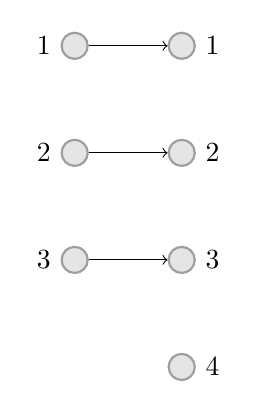
\begin{tikzpicture}[place/.style={circle,draw=darkgray!50,fill=gray!20,thick}]
       \node[place,label=left:1] (one3) {};
       \node[place,label=left:2] (two3) [below=of one3] {};
       \node[place,label=left:3] (three3) [below=of two3] {};

       \node[place,label=right:1] (one4) [right=of one3] {};
       \node[place,label=right:2] (two4) [below=of one4] {};
       \node[place,label=right:3] (three4) [below=of two4] {};
       \node[place,label=right:4] (four4) [below=of three4] {};

       \draw [->] (one3) to [thick, shorten <=1pt,>=stealth'] (one4);
       \draw [->] (two3) to [thick, shorten <=1pt,>=stealth']  (two4);
       \draw [->] (three3) to [thick, shorten <=1pt,>=stealth']  (three4);
    \end{tikzpicture}}
\hspace{7.5em}
  \subfigure[]{
  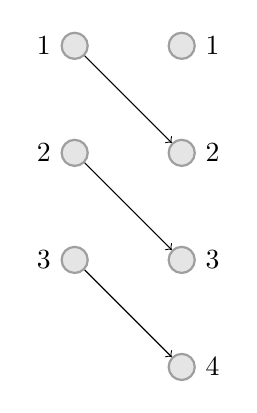
\begin{tikzpicture} [place/.style={circle,draw=darkgray!50,fill=gray!20,thick}]
       \node[place,label=left:1] (one3) {};
       \node[place,label=left:2] (two3) [below=of one3] {};
       \node[place,label=left:3] (three3) [below=of two3] {};

       \node[place,label=right:1] (one4) [right=of one3] {};
       \node[place,label=right:2] (two4) [below=of one4] {};
       \node[place,label=right:3] (three4) [below=of two4] {};
       \node[place,label=right:4] (four4) [below=of three4] {};

       \draw [->] (one3) to [thick, shorten <=1pt,>=stealth'] (two4);
       \draw [->] (two3) to [thick, shorten <=1pt,>=stealth']  (three4);
       \draw [->] (three3) to [thick, shorten <=1pt,>=stealth']  (four4);
  \end{tikzpicture}}

\vspace{4ex}
\caption{The graph of the |inject| function (a) and the |raise|
  function (b) embedding |Fin 3| in |Fin (3 + 1)|}
  \pepijn{Thanks, this is MUCH more readable. :)}
  \label{fig:fins}
\end{figure}

Using |inject| and |raise| as defined to work on finite sets, we can
define similar functions that work on our |Rule| and |Term| data
types.



\subsection{Proof search}

Our implementation of proof search is divided up into two steps.
In the first step we set up an abstract representation of the search
space in which we implement the basic machinery of sequential rule
application.
In the second step we make transform this abstract representation into
a concrete search tree by introducing a set of rules.

The reason we have chosen to separate these two steps is that it
neatly separates the machinery for proof search (be it breath-first
search, depth-first search or some heuristic-driven algorithm) from
the machinery for unification.

%\subsubsection{Setting up the search space}

\begin{code}
  data SearchSpace (m : ℕ) : Set where
    done : (∃₂ δ n → Subst (m + δ) n) → SearchSpace m
    step : (∃ Rule → ∞ (SearchSpace m)) → SearchSpace m
\end{code}

%\subsubsection{Searching the search space}

\begin{code}
  data SearchTree (A : Set) : Set where
    fail : SearchTree A
    retn : A → SearchTree A
    fork : ∞ (List (SearchTree A)) → SearchTree A
\end{code}


\section{Constructing proof trees}
\label{sec:proofs}

\section{Adding reflection}
\label{sec:reflection}


\section{Extended example}
\label{sec:example}

\todo{Give a bigger example of debugging/automated proving}

\section{Discussion}
\label{sec:discussion}

\todo{Mention Idris}

Future work: auto rewrite; setoid rewrite; proof combinators.

limitations of using recursion in hint data base

Cf Agsy



Combining hint data bases

Debugging failed auto attempts, or other examples from
\url{http://adam.chlipala.net/cpdt/html/LogicProg.html}

We cannot `insert goals' in the term produced by a call to auto. This
could be useful if you want to allow a tactic to return an unfinished
proof. Or can we?

Work with \emph{typed} term language. This is a hard problem.

Compare with Mtac.

Cite Devriese paper.

\bibliographystyle{plainnat}
\bibliography{main}

\end{document}

%%% Local Variables:
%%% mode: latex
%%% TeX-master: t
%%% TeX-command-default: "rake"
%%% End:
